\documentclass{homeworg}
\usepackage{amsmath}

\title{Travail 1 - Circuits DC}
\author{Wats Raphaël}

\begin{document}
\maketitle

\section{Schéma du circuit}
    \begin{center}
        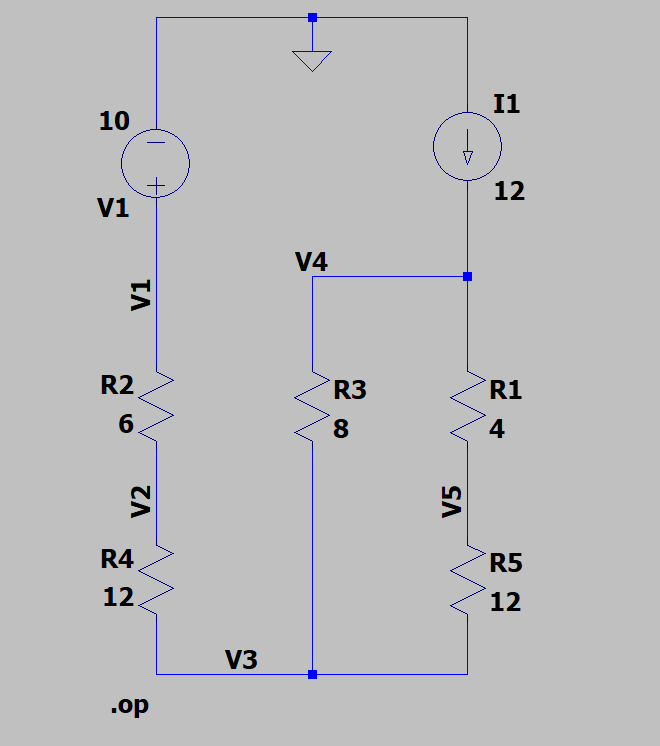
\includegraphics[scale=0.7]{Shematic.PNG}
    \end{center}

\section{Détail des calculs}
    \begin{center}
        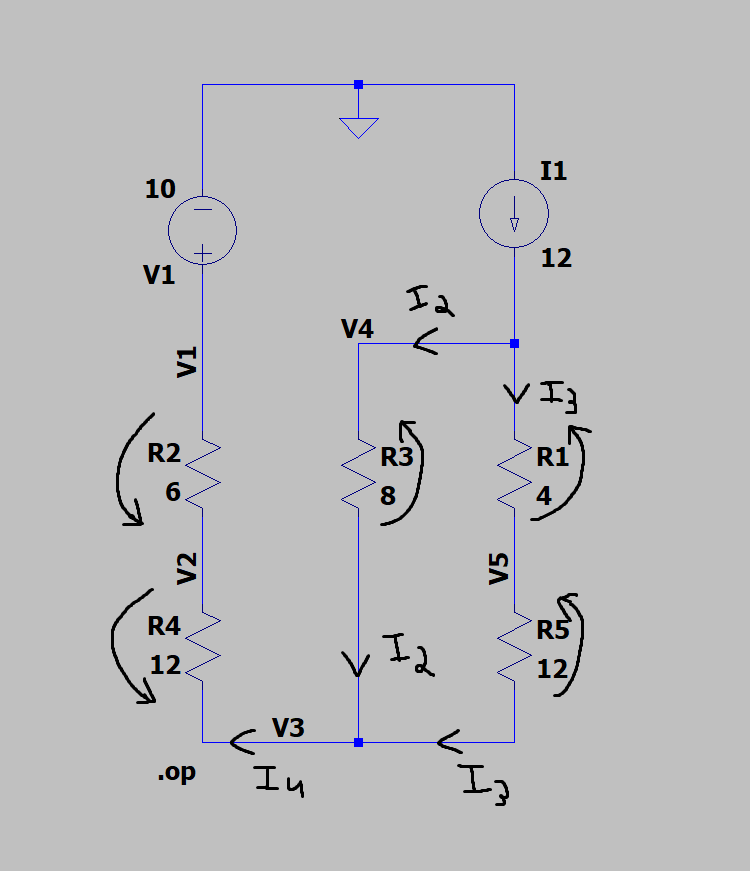
\includegraphics[scale=0.5]{Calculs.png}\\
        \large
        Calcul des courants et tensions
    \end{center}
    \normalsize
    \begin{align}
        I_1 = I_2 + I_3\\
        I_4 = I_2 + I_3\\
        I_1 = I_4 = 12 \\
        I_4 = (V_2 - V_1) / R_2 = (V_2 - 10) / 6 = 12\\
        V_2 = (6 * 12 + 10) = 82\\
        I_4 = (V_3 - V_2) / R_4 = (V_3 - 82) / 12 = 12\\
        V_3 = 12 * 12 + 82 = 226\\
        I_3 = (V_4 - V_5) / R_1 = (V_4 - V_5) / 4\\
        I_3 = (V_5 - V_3) / R_5 = (V_5 - 226) / 12\\
        (V_4 - V_5) / 4 = (V_5 - 226) / 12\\
        V_5 = (3V_4 + 226) / 4\\
        I_2 = (V_4 - V_3) / R_3 = (V_4 - 226) / 8\\
        I_1 = (V_4 - V_3) / R_3 + (V_5 - V_3) / R_5 =
        (V_4 - V_3) / R_3 + ((3V_4 + 226) / 4 - V_3) / R_5\\
        I_1 = (V_4 - 226) / 8 + ((3V_4 + 226)/4 - 226)/12\\
        V_4 = 5220 / 18 = 290\\
        V_5 = (3 * 290 + 226) / 4 = 274\\
        I_2 = (290 - 226) / 8 = 8\\
        I_3 = (290 - 274) / 4 = 4
    \end{align}
    \newpage
    \begin{center}
    \large
        Calcul des puissances
    \end{center}
    
    \normalsize
    \begin{align}
        P_{I1} = (GROUND - V_4) * I1 = (0 - 290) * 12 = -3480\\
        P_{V1} = (V_1 - GROUND) * I4 = 10 * 12 = 120\\
        P_{R1} = (V_4 - V_5) * I_3 = (290 - 274) * 4 = 64\\
        P_{R1} = (V_2 - V_1) * I_4 = (82 - 10) * 12 = 864\\
        P_{R3} = (V_4 - V_3) * I_2 = (290 - 226) * 8 = 512\\
        P_{R4} = (V_3 - V_2) * I_4 = (226 - 82) * 12 = 1728\\
        P_{R5} = (V_5 - V_3) * I_5 = (274 - 226) * 4 = 192\\
        P_{total} = P_{I1} + P_{V1} + P_{R1} + P_{R2} + P_{R3} + P_{R4} + P_{R5} = 0
    \end{align}

\section{Conclusion}
    Les résultats obtenu sont en adéquation avec ceux obtenu lors de la simulation LTspice XVII.
    \begin{center}
        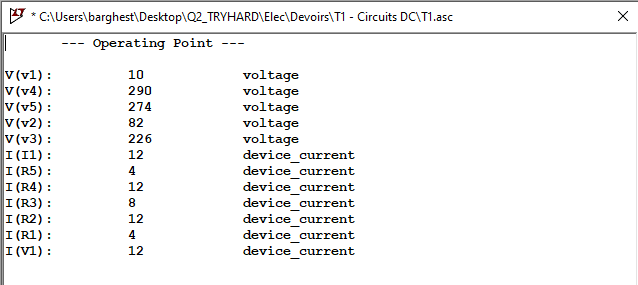
\includegraphics[scale=0.75]{Results.PNG}
    \end{center}
    \begin{itemize}
        \item La somme des courants entrant d'un noeud est bel et bien égale à la somme des courants sortant de ce même noeud.
        \item La somme des puissances fournies total est bel et bien égale à somme des puissances dissipées total.
    \end{itemize}
\end{document}
